\section{Recaudaciones para papá fisco}
Una empresa de ayudantías de Python organizada por unos ayudantes organiza la cobranza de sus clientes en dos archivos de texto: \texttt{clientes.txt} y \texttt{descuentos.txt}, ambas con líneas de forma \texttt{nombre: monto\_neto}.

\begin{figure}[h]
    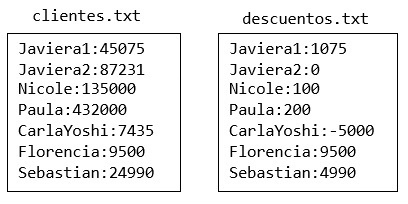
\includegraphics{Guia/imagen2.jpg}
\end{figure}

Se le pide a usted crear el archivo \texttt{brutos.txt} que indicará el nombre del cliente, monto neto, descuento, y valor final, separados por dos puntos. Entiéndase que el valor final se calcula agregando el IVA a la diferencia del monto neto y el descuento.
\begin{displaymath}
valor final = (monto neto - descuento) * 1.19
\end{displaymath}

\paragraph{Aclaraciones} Cualquier parecido con la realidad es mera coincidencia.